% Chapter 4
\chapter{Transmission Expansion Planning by Quantum Annealing} % Main chapter title
\label{Chapter4} % For referencing the chapter elsewhere, use \ref{Chapter1} 
\section{Statement of the problem}
\begin{wrapfigure}{l}{0.35\textwidth}
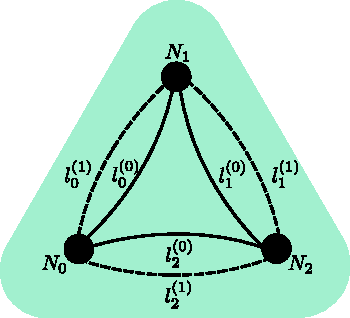
\includegraphics[scale=0.9]{Figures/3Node_Layer 1.pdf} 
\caption{An example considering a three node transmission expansion planning (TEP) problem with three candidate lines. Solid lines represent existing lines (super-index $(0)$) and dash lines are the candidate lines (super-index $(1)$).}
\label{fig:3node}
\end{wrapfigure}
\textit{Transmission expansion planning} (TEP)\,\cite{Neumann2020TransmissionFlows} is a \textit{mixed integer linear problem} (MILP) that aims at finding the optimal way to expand the capacity of an energy system. It decides how many components to build in order to satisfy the energy demand on a distributed energy system with a high share of renewable energy sources. Often these problems of improving the existing network to fulfill future targets are taken into account together under the name of transmission expansion planning but in this case we are just considering transmission lines which reduce drastically the number of variables involved. Reducing the number of variables allow us to solve the whole problem with a quantum annealer. However, this reduction in complexity implies that the problem we are solving is not realistic and we should consider it as our starting point. \\\\
The TEP scales badly using classical algorithms\,\cite{Oertel2014ComplexityEvaluation} and, at the same time, energy system models are getting larger and more complex due to the integration of decentralized weather-dependent renewable energy sources, sector coupling and the increase of storage components.\\\\
Currently, the problem is often linearized or the scope and granularity of the model are reduced using clustering algorithms. For this reason, any computational time reduction will have substantial implications in closing the granularity gap between what the current models can solve and the desired resolution needed by energy system operators. We plan to scale the problem by increasing the number of nodes, targets to fulfill and the candidate components to build such as storage or generators of different carriers (wind turbines, heat pump, solar panels and so on), but with the current maturity of quantum annealers such problems are not solvable. We require of hybrid methods\,\cite{Zhao2021HybridProgrammingb} to decompose the problem into a master problem which can be solved by a quantum annealer and a sub-problem for which cutting-edge classical algorithms are going to be applied. There is already a paper on the application of hybrid quantum-classical algorithms\,\cite{Paterakis2021HybridApplication} with a power system application using Benders' Decomposition techniques, concretely multi-cuts, but we plan to apply single-cut Benders' decomposition to the problem exploring how can a TEP problem be benefited from quantum annealing in the future.\\\\
\begin{wraptable}{R}{7.2cm}
\centering
\begin{tabular}{cc} \\\toprule 
 \textbf{Symbol} & \textbf{Description} \\\midrule
 $\mathcal{N}$ & Nodes  \\\midrule
 $\mathcal{L}^{(0)}$ & Existing transmission lines  \\\midrule
 $\mathcal{L}^{(1)}$ & Candidate transmission lines \\\midrule
 $\mathcal{D}_{i}$ & Demand of node $i$. \\\midrule
 $\mathcal{G}_{i}$ & Energy generation at node $i$. \\\midrule
 $\mathcal{T}_{i}$ & Transmission Capacity of line $i$. \\\midrule
 $\mathcal{C}_{i}$ & Investment cost of line $i$ \\\bottomrule 
\end{tabular}
\caption{Nomenclature.}
\label{table:TEPNomenclature}
\end{wraptable}
We start by considering a small network of three nodes $N_{i}\in \mathcal{N}$ with 3 existing lines $l_{i}^{(0)}\in \mathcal{L}^{(0)}$ and 3 candidate lines $l_{i}^{(1)}\in \mathcal{L}^{(1)}$, (Figure \ref{fig:3node}). The nodes can be though as towns whose energy demand has to be fulfilled and the lines allow the network to transmit energy between nodes so that if some node is producing more energy than its demand, then that excess of energy can be transmitted to other node of the network. For now we are going to focus on the ability of each node in transmitting energy to other node assuming a set of snapshots is given, i.e., in each snapshot a node will require energy from the other two nodes. Our task is to fulfill this energy transmission demand between nodes so that our investment cost is minimum.
%%%%%%%%%%
\section{QUBO formulation of three-node TEP}
The objective function of TEP is
\begin{equation}
    \min_{\vec{l}^{1)}}\sum_{i=0}^{2}\mathcal{C}_{i}l_{i}^{(1)}
\end{equation}
subject to,
\begin{equation}
    \mathcal{D}_{j} = \sum_{i=0}^{2}\mathcal{T}_{i}^{(0)}l_{i}^{(0)} + \sum_{i=0}^{2}\mathcal{T}_{i}^{(1)}l_{i}^{(1)}, \quad \forall j \in \left[0,1,2\right] 
\end{equation}
where each $j$ is a snapshot. For simplicity each snapshot correspond to a single node demand labelled with the same index. \par
The numerical values are
\begin{align}
\vec{\mathcal{C}} =
        \begin{bmatrix}
           1  \\
           3  \\
           4
         \end{bmatrix} \\
\vec{\mathcal{D}} =
        \begin{bmatrix}
           5  \\
           7  \\
           7
         \end{bmatrix} \\
         \mathcal{T}_{i} = 3 , \quad \forall i
\end{align}
The number of slack variables required for the constraints is given by,
\begin{align}
    M_{0} = \lfloor\log_{2}{\mathcal{D}_{0}}\rfloor = 2 \\
    M_{1} = \lfloor\log_{2}{\mathcal{D}_{1}}\rfloor = 2 \\
    M_{2} = \lfloor\log_{2}{\mathcal{D}_{2}}\rfloor = 2
\end{align}
where,
\begin{align}
    \mathcal{D}_{0} = \sum_{k=0}^{M}c_{k}^{0)}y_{k}^{0)} \\
    \mathcal{D}_{1} = \sum_{k=0}^{M}c_{k}^{1)}y_{k}^{1)} \\
    \mathcal{D}_{2} = \sum_{k=0}^{M}c_{k}^{2)}y_{k}^{2)}
\end{align}
with $c_{M}^{j)} = D_{j} + 1 - 2^{M}$. Now we can include the constraints into the cost function via penalties
\begin{align}
    \min_{\vec{l}^{1)},\vec{y} }\sum_{i=0}^{2}\mathcal{C}_{i}l_{i}^{(1)} + P_{0}\left[\sum_{k=0}^{M}c_{k}^{0)}y_{k}^{0)} - \sum_{i=0}^{2}\mathcal{T}_{i}^{(0)}l_{i}^{(0)} + \sum_{i=0}^{2}\mathcal{T}_{i}^{(1)}l_{i}^{(1)}\right]^{2} \\
    + P_{1}\left[\sum_{k=0}^{M}c_{k}^{1)}y_{k}^{1)} - \sum_{i=0}^{2}\mathcal{T}_{i}^{(0)}l_{i}^{(0)} + \sum_{i=0}^{2}\mathcal{T}_{i}^{(1)}l_{i}^{(1)}\right]^{2}\\
    + P_{2}\left[\sum_{k=0}^{M}c_{k}^{2)}y_{k}^{2)} - \sum_{i=0}^{2}\mathcal{T}_{i}^{(0)}l_{i}^{(0)} + \sum_{i=0}^{2}\mathcal{T}_{i}^{(1)}l_{i}^{(1)}\right]^{2}  
\end{align}
We can assign the same penalty to each constraint as all constraints are analogous $P = P_{0} = P_{1} = P_{2}$.\\
We expand one square to demonstrate how to formulate QUBO problems. To simplify the notation we drop the indices and rename the constant $K = \sum_{i=0}^{2}\mathcal{T}_{i}^{(0)}l_{i}^{(0)}$
\begin{align*}
    \left(c_{0}y_{0} + c_{1}y_{1} + c_{2}y_{2} - K + Tl_{0}+ Tl_{1} + Tl_{2}\right)^{2} = \\
    y_{0}c_{0}^{2}y_{0} + y_{0}2c_{0}c_{1}y_{1} + y_{0}2c_{0}c_{2}y_{2} + y_{0}2c_{0}Tl_{0} + y_{0}2c_{0}Tl_{1} + y_{0}2c_{0}Tl_{2} - y_{0}2Kc_{0}y_{0}\\
    y_{1}c_{1}^{2}y_{1} + y_{1}c_{1}c_{2}y_{2} + y_{1}2Tc_{1}l_{0} + y_{1}2Tc_{1}l_{1} + y_{1}2Tc_{1}l_{2} - y_{1}2Kc_{1}y_{1}\\
    y_{2}c_{2}^{2}y_{2} + y_{2}2Tc_{2}l_{0} + y_{2}2Tc_{2}l_{1} + y_{2}2Tc_{2}l_{2} - y_{2}2Kc_{2}y_{2}\\
    l_{0}T^{2}l_{0} + l_{0}2T^{2}l_{1} + l_{0}2T^{2}l_{2} - l_{0}2KTl_{0}\\
    l_{1}T^{2}l_{1} + l_{1}2T^{2}l_{2} - l_{1}2KTl_{1}\\
    l_{2}T^{2}l_{2} - l_{2}2KTl_{2} 
\end{align*}
Notice that constant terms $K^{2}$ are dropped because they do not modify the configuration at which the minimum value of cost function is. \\
Finally the QUBO matrix of this problem is,
\begin{equation}
Q =
        \begin{bmatrix}
           3T^{2} & 6T^{2} & 6T^{2} & 2T & 4T & 2T & 2T & 4T & 8T &2T & 4T & 8T  \\
           0 &3T^{2}& 6T^{2} & 2T & 4T & 2T & 2T & 4T & 8T &2T & 4T & 8T \\
           0 & 0 & 3T^{2} &2T & 4T & 2T & 2T & 4T & 8T &2T & 4T & 8T \\
           0 & 0 & 0 & 1 & 4 & 4 & 0 & 0 & 0 & 0 & 0 & 0\\
           0 & 0 & 0 & 0 & 4 & 8 & 0 & 0 & 0 & 0 & 0 & 0\\
           0 & 0 & 0 & 0 & 0 & 4 & 0 & 0 & 0 & 0 & 0 & 0\\
           0 & 0 & 0 & 0 & 0 & 0 & 1 & 4 & 8 & 0 & 0 & 0\\
           0 & 0 & 0 & 0 & 0 & 0 & 0 & 4 & 16& 0 & 0 & 0\\
           0 & 0 & 0 & 0 & 0 & 0 & 0 & 0 & 16& 0 & 0 & 0\\
           0 & 0 & 0 & 0 & 0 & 0 & 0 & 0 & 0 & 1 & 4 & 8 \\
           0 & 0 & 0 & 0 & 0 & 0 & 0 & 0 & 0 & 0 & 4 & 16\\
           0 & 0 & 0 & 0 & 0 & 0 & 0 & 0 & 0 & 0 & 0 & 16
         \end{bmatrix}
\end{equation}
\section{Running QUBO problem on D-WAVE's annealer}
\subsection{Three-Node without discretization in transmission capacities}
In this example we solved the three-node network with three candidate lines where the transmission capacities are fixed, i.e., if a line transmit electricity it does it always with the same value. In this way we can simplify the problem by not using slack variables for discretizing the transmisssion capacities.
%%%%%%%%%%%%%%%%%%%%%%%%%%%%%%%%%%%%%%%%%%%%%%%%%%%%%%%%%%%%%%%%%%%%%%%%%%%%%
% Hybrid Classical-Quantum annealing
%%%%%%%%%%%%%%%%%%%%%%%%%%%%%%%%%%%%%%%%%%%%%%%%%%%%%%%%%%%%%%%%%%%%%%%%%%%%%

We can scale the problem by taking into account,
\begin{itemize}
    \item \textbf{Snapshots of time}: In expansion problems is common to consider hourly snapshots of time of one year.
    \item \textbf{Adding transmission lines}: It does not make sense to build an isolated generator. We need transmission lines to connect different nodes of a network. Solving both problems at the same time reduce the total cost as compared with solving each one individually.
    \item \textbf{Adding targets}: In the present project we a single target, i.e., the cost function -- investment and operational cost -- but there are other targets such are increase the percentage of renewable sources in a given region or reducing the carbon footprint that are also common among expansion planning models.
\end{itemize}